\section{Proofs of Lemmas \ref{lem:s1Small} through \ref{lem:disksOfPathways}}
We now prove the Lemmas \ref{lem:s1Small} through \ref{lem:disksOfPathways}.
\subsection{Proof of Lemma \ref{lem:s1Small}}
\begin{proof}
Recall that we are to show that for any realized perturbed snowflake $S_i$, the gaps created in subset $S_1 \subset S_i$ are small.  

\begin{minipage}{\linewidth}
\begin{center}
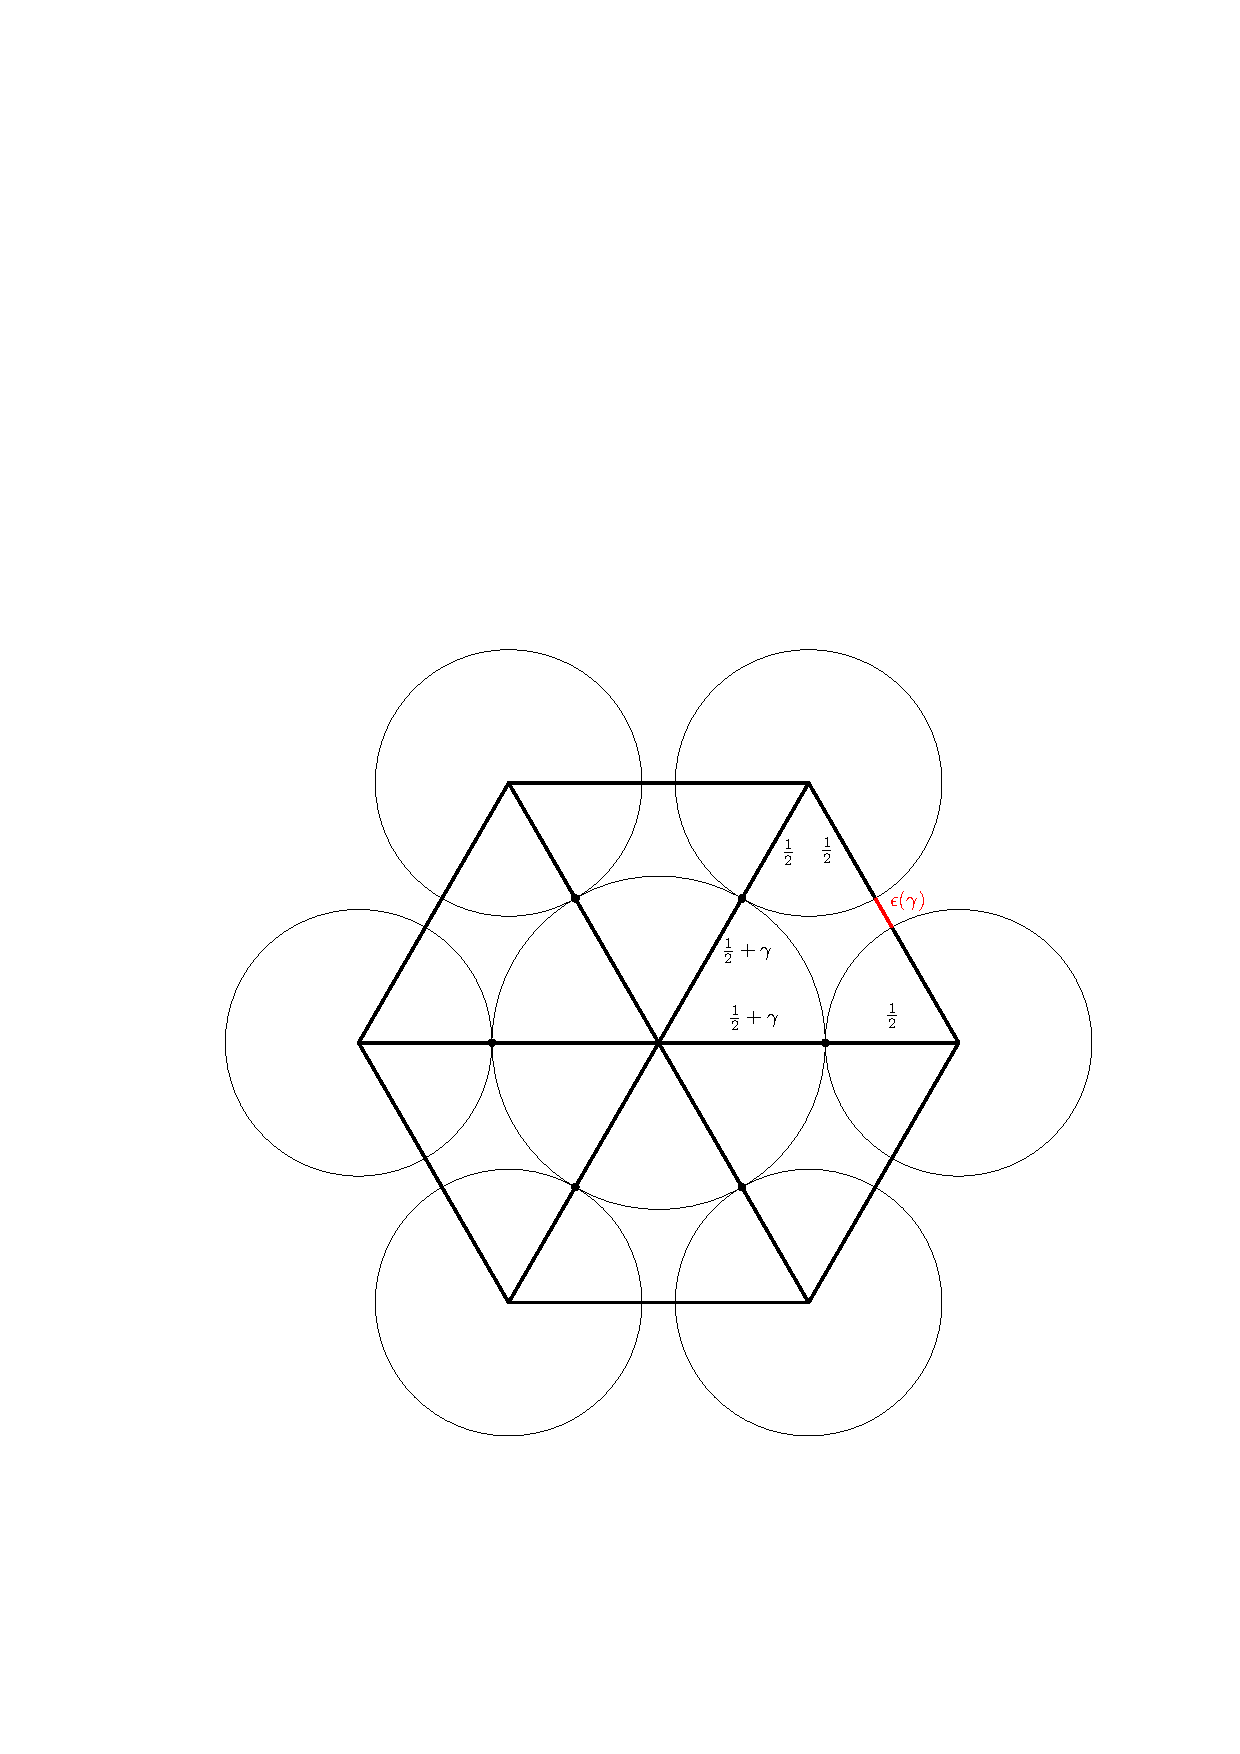
\includegraphics[width=.33\columnwidth]{graphics/modifiedContactGraph.pdf}
\captionof{figure}{A canonical disk arrangement from a perturbed snowflake with 6 unit disks around a central disk with radius $\frac{1}{2} + \gamma$.}\label{fig:modifiedContactGraph.pdf}
\end{center}
\end{minipage}

One way to do this is to demonstration that the sum of gaps for any realization of a contact graph of a perturbed snowflake $S_1$ is small. 
Denote the vertices around $v_0$ as $v_1$ through $v_6$ in a clockwise pattern about $v_0$. 
Without loss of generality, given a realization denote $\epsilon_{k, k+1} (\gamma)\geq 0$ as the gap created between adjacent disks corresponding to $v_1$ thourgh $v_6$.

Consider the realization where $\epsilon_{k, k+1} (\gamma) = 0$ with the exception of $\epsilon_{1,6} >0$.  
That is, ever consecutive pair of disks about the central disk is in contact with each other with the exception of $D_1$ and $D_6$.  
The realization provides 5 congruent triangles between the centers of $D_0$ and $\lr{D_1,D_2}$, $\lr{D_2,D_3}$, $\lr{D_3,D_4}$, $\lr{D_4,D_5}$, and $\lr{D_5,D_6}$.  
Given perturbation $\gamma > 0$, the side lengths between $\lr{D_0,D_i}$ are $1 +\gamma$ and the side length of $\lr{D_i, D_{i+1}}$ is 1.
Using law of cosine the angle formed between $\lr{D_0,D_i}$ and $\lr{D_0,D_{i+1}}$ is $$2 \tan^{-1} \frac{1}{2\lr{1+\gamma}}.$$  
The angle between $\lr{D_6, D_1}$ is $$y=2 \pi - 5 \cdot \lr{2 \tan^{-1} \frac{1}{2\lr{1+\gamma}}}.$$  
The side length of $\lr{D_6, D_1}$ is
$$\sqrt{-2 \, {\left(\gamma + 1\right)}^{2} \cos\left(-10 \,
\arctan\left(\frac{1}{2 \, {\left(\gamma + 1\right)}}\right)\right) + 2
\, {\left(\gamma + 1\right)}^{2}}.$$
Note that as $\gamma \rightarrow 0$, the side length of $\lr{D_6, D_1}$ is approximately 1 + .466861, where $\epsilon(\gamma) \approx .466861$ as $\gamma \rightarrow 0$.
This establishes an upperbound on the maximal displacement about $S_1$ with respect to the side lengths between the centers of disks about $D_0$.

The lower bound is established using the configuration found in Figure \ref{fig:modifiedContactGraph.pdf}.  
he realization provides 6 congruent triangles between the centers of $D_0$ and each disk about $D_0$.
Without loss of generality, to find the side length of between neighboring disks about $D_0$, we find need to $\epsilon(\gamma)$.  
The angle between $\lr{D_0, D_i}$ and $\lr{D_0,D_{i+1}}$ is $\frac{\pi}{3}$; using the law of cosine, we can determine the side length of $\lr{D_i,D_{i+1}}$ is $$\sqrt{1 + 2 \gamma + \gamma^2}.$$  


Thus the perturbation about $S_1$ in and confiugration is bounded and small.
\end{proof}
\subsection{Proof of Lemma \ref{lem:angularArrangement}}
\begin{proof}
Recall that we are to show that for any realized perturbed snowflake $S_i$, the angular value of $\alpha_k$ and $\beta_k$ are small.  
In canoncical position, the angle between $p_{k,j}^+$ and $p_{k,j}^-$ is $\frac{\pi}{3}$.  
In a non-canonical position, we define the change in angle to be $f(\epsilon)$.  
About a 
We prove this with induction. 


\begin{minipage}{\linewidth}
\begin{center}
\includegraphics[width=.66\columnwidth]{graphics/Vertebrae.pdf}
\captionof{figure}{}\label{fig:Vertebrae.pdf}
\end{center}
\end{minipage}

% First consider the changes the angles $\alpha_1$, $\beta_1$, $\alpha_2$, and $\beta_2$.  
$$
\begin{array}{rcl}
\alpha_i +\beta_i &\leq& 120 + f(\epsilon)\\
2 \pi &\leq& \gamma_i + \delta_i + \frac{2 \pi}{3} + f(\epsilon)\\
2 \pi - \lr{\gamma_i + \delta_i} &\leq& \frac{2 \pi}{3} + f(\epsilon)\\
\alpha_{i+1} + \beta_{i+1} &\leq& \frac{2 \pi}{3} + f(\epsilon)\\
\end{array}
$$
\end{proof}
\subsection{Proof of Lemma \ref{lem:disksOfPathways}}
\begin{proof}
Recall that we are to show that for any realized perturbed snowflake $S_i$, the distance between disks $D_{k,j}$, $D_{k+1,j}$, $D_{k+1,j+1}$, and $D_{k,j+1}$ are relatively small with respect to the relative distance in a perfect snowflake where $k = 1$, $\dots$, $6$ and $j = 2$, $\dots$, $i$.

\begin{minipage}{\linewidth}
\begin{center}
\includegraphics[width=.66\columnwidth]{graphics/ch4Paralellogram.pdf}
\captionof{figure}{}\label{fig:ch4Paralellogram.pdf}
\end{center}
\end{minipage}


\end{proof}